\documentclass[12pt,letterpaper]{article}

\usepackage{amsmath, amsthm}
\usepackage{microtype, parskip}
\usepackage[comma,numbers,sort&compress]{natbib}
\usepackage{lineno}
\usepackage{docmute}
\usepackage{caption, subcaption, multirow, morefloats, rotating}
\usepackage{wrapfig}
\usepackage{attrib}

\frenchspacing

\begin{document}

\section*{Introduction}
A regional species pool is the set of species which form communities in a specific region \citep{Mittelbach2015a,Harrison2008}. Local scale processes like resource competition only affect the regional species pool if all communities are affected. The taxonomic and functional composition of a regional species pool changes over time due to speciation, migration, and extinction. How do species pools change over time as species are recruited or go extinct? When are specific species ecologies enriched or depleted in the species pool? How does global and regional environmental context affect the set of species ecotypes (e.g. guilds) in a regional species pool? I address these questions through an analysis of the ecological and functional diversity of North American mammals for most of the Cenozoic, or last 65 million years.

% guilds and ecocube and ecotypes
Functional diversity is frequently thought of as a set of guilds, which themselves are a set of species with similar sets of interactions and interactors (i.e. macroecology) \citep{Valentine1969,Bambach1977,Brown1989,Simberloff1991a,Wilson1999}. Species within a guild are expected to have more similar macroecological dynamics than species in a different guilds. Building on the concept of guilds and a macroecological niche, \citet{Bush2007} presented a three-dimensional construct, or ecocube, for describing the macroecological role of a marine invertebrate species by their physical position (i.e. tiering), motility, and trophic role. Unique combinations along the three ecological trait axes indicate which among the possible ecotypes are observed. This approach has proven quite popular as it attempts to operationalize the guild concept in terms of shared characteristics that are indicative of the type of interactions experience by species of that macroecology \citep{Bush2007,Bambach2007,Bush2011,Bush2012b,Novack-Gottshall2007,Villeger2011}, but the utility of this approach is limited due to its condition as just a data type.

% how we think about mammal diversity
Previous analysis of mammal diversity and hypotheses as to the processes that have shaped it tend to be through one or more of the following lenses: diversity of an entire system (e.g. continent) \citep{Alroy2000g,Alroy1996a,Figueirido2012,Liow2008}, guild based \citep{Janis2004,Janis2000,Jernvall2004,Janis1993c,Pires2015a,Janis2008a}, clade based \citep{Quental2013,Slater2015c,Silvestro2015b,Fraser2015a,Cantalapiedra2017}, and environment based \citep{Blois2009,Janis1993c,Janis1993b,Fraser2015a,Eronen2015,Badgley2013,Badgley2017}. Rarely are more than two of these lenses considered simultaneously, and integration across the resulting diversity of observations and hypotheses tends to be based on coincidence. One of the goals of this study is to present a framework for simultaneously analyzing a diversity of hypotheses by integrating both species traits and environmental factors into a single model in order to infer a more holistic multi-level picture of the processes which may have shaped mammal species diversity and diversification.

% what we're dealing with in terms of hypotheses
The principle species trait considered in this study is a species' ecotype, defined here as the unique combination of dietary cateogry and locomotor category (e.g. arboreal omnivore versus unguligrade herbivore). These classifications can be considered analogous to guilds or unique ecocube combinations as discussed above \citep{Bush2007,Bambach2007,Bush2011}. Species mass was also included as a species trait, but its inclusion is principally to control for that effect on the other covariates that are the focus of this study.

Translating previous work into hypotheses applicable to this analysis is difficult for a variety of reasons. Taxonomic groupings such as order or family are frequently invoked as an important factor in many proposed hypotheses for how mammal diversity is structured \citep{Quental2013,Slater2015c,Janis1993c,Pires2015a,Janis2008a}. Because taxonomic grouping conflates both species macroecology with shared evolutionary history, there are few clear ways to translate and operationalize these hypotheses in terms of macroecological change viewed through the lens of species interactions. Specifically, this issue arrises when trying to generalize previous observations from taxony-based framework to ecology-based one.

There is little convincing evidence of any major or sudden cross-ecotypic or cross-taxonomic turnover events in history of North American mammal diversity, unlike the Neogene record European mammals \citep{Alroy2009,Alroy1996a,Eronen2015,Janis1993b,Alroy2000g}. Instead of being concentrated in time, turnover has been found to be distributed through time. It is then expected then that, for this analysis, turnover events or periods of rapid diversification or depletion should not occur simultaneously for all ecotypes.

\citet{Jernvall2004} found that for the Neogene of Europe the relative abundance of mammal guilds was stable over time even in the face of high turnover rates, though they only considered large bodied taxa from a small set or mammal orders. Similar results have been observed for some taxonomic groups in North America \citep{Valkenburgh1999}. These results imply that there the types of interactions happening in local communities observed over a region are constant over time even if the interactors are constantly changing. A diversity-dependent or somehow limited diversification history is also theorized for North American mammal diversity as a whole \citep{Alroy2009,Rabosky2015b}, though the evidence for this is limited \citep{Harmon2015a}.

The diversity history of ungulate herbivores has been characterized by more recently originating taxa having longer legs, higher crowned teeth, and a shift from graze-dominated to browse-dominated diets than their earlier originating counterparts \citep{Janis2004,Janis2000,Janis1993c,Janis2008a,Cantalapiedra2017,Fraser2015a}; all of which has all been attributed to some combination of tectonic activity driving environmental change or environmental change itself \citep{Janis2008a,Eronen2015,Blois2009,Badgley2017}. Additionally, it has been observed that these cursorial ungulate forms arose prior to cursorial carnivore forms, an observation attributed to the reorganization of plant communities towards the end of the Cenozoic and the latter emergence of ``modern'' environments and communities \citep{Janis1993c}.

Within the canid guild of North America (e.g. plantigrade and digitigrade carnivores) there is evidence that their diversity is self-regulating or somehow limited \citep{Valkenburgh1999}. Specifically, it has been proposed that different canid clades have replaced each other as the dominate members of that macroecological role within the species pool \citep{Silvestro2015b}. A pattern of generally constant diversity through time is also observed within the canid carnivore subguilds of hypercarnivore, hypocarnivore, and mesocarnivores identified by \citet{Slater2015c} even in the face of constant species turnover is consistent with limited possibility of increased diversity, even though there was no evidence of diversity-dependence in trait (e.g. body size) evolution \citep{Slater2015c}.

There is some uncertainty and a lack of consensus as to the effect of species body size on mammal diversity and aspects of the diversification processes, specifically extinction \citep{Liow2008,Liow2009,Tomiya2013,Smits2015b}. Species body size is frequently framed as an important biological descriptor because of its correlation with other important and relevant ecological traits such as metabolic rate and home range size \citep{Brown1995}. It is also relatively easy to estimate for extinct species using proxy measures and regression equations, as was done in this study (see below). However, body size is normally analyzed without simultaneous reference to other species traits \citep{Liow2008,Huang2017,Raia2012f,Smith2004}, but see \citep{Smits2015b}; this combined with the high amount of correlation between life history traits and body size limits processed-based inference because the actual causal mechanisms underlying an observed pattern are obscured or missing.

\citet{Smits2015b} found that the individual traits which form this study's ecotypes have strong effects on mammal extinction risk. Omnivorous taxa were found to have, on average, a greater duration than other dietary categories, while arboreal taxa were found to have a shorter duration than other locomotor categories \citep{Smits2015b}. Two possible scenarios that could yield this pattern were proposed: the extinction risk faced by arboreal is constant and high or the Paleogene and Neogene represent different regimes and extinction risk increased in the Neogene, thus driving up the Cenozoic average extinction risk. These two possible explanations have clear and testable predictions with respect to the diversity history of arboreal taxa: 1) the extinction risk arboreal taxa increased in the Neogene compared to the Paleogene, driving the average extinction risk of arboreal mammals up and leading to the loss of arboreal taxa from the species pool, or 2) if arboreal taxa have just a generally higher extinction risk than other ecotypes but have maintained a constant diversity for the Cenozoic. By inspecting the inferred diversity histories of the ecotypes, it should be possible to distinguish amoungst these hypotheses.

% if we control for one ecotype axis, what is variation along other axis?
% digitigrade vs unguligrade herbivores
% plantigrade vs digitigrade carnivores
% modernization of ecologies?
%   this is normally talked about in terms of taxonomic groups
%   how does this translate into ecologies?




% effect of climate on diversification process
Fundamentally, all species respond differently to climate and environmental change \citep{Blois2009}. Macroecological patterns are emergent patterns due to the similarities among species in how they respond to a similar ``stimulus.''

The effect of climate on diversity and the diversification process has been the focus of considerable research with a slight consensus favoring diversification being more biologically-mediated than climate-mediated \citep{Alroy1996a,Alroy2000g,Figueirido2012,Clyde1998a}. However, differences in temporal and geographic scale seem to underly the contrast between these two perspectives. For example when the mammal fossil record analyzed at small temporal and geographic scales a correlation between diversity and climate are observable \citep{Clyde1998a}. However, when the record is analyzed at the scale of the continent and most of the Cenozoic there is no correlation with diversity and climate \citep{Alroy2000g}. This results, however, does not go against the idea that there may be short periods of correlation and that the correlation between diversity and climate can change or even reverse direction over time; this type result means that there is no single direction of correlation between diversity and climate \citep{Figueirido2012}. 

In the case of a fluctuating correlation between diversity and climate it is hard to make the argument for an actual causal link between the two without modeling the underlying ecological differences between species; after all, species respond differently based on their individual ecologies \citep{Blois2009}. When analysis is based on diversity or taxonomy alone no mechanisms are possible to infer. Taxonomy, like body size, stands in for many important species traits to the point that mechanistic or process based inference is impossible. While emergent patterns might correspond to taxonomic grouping, this itself is an emergent phenomenon. Instead, by framing hypotheses in terms of species traits and their environmental context, these emergent phenomenon can be observed rather than assumed.

The climate history of the Cenozoic is generally characterized by a global cooling trend and the development of polar ice-caps during the Neogene; there are, of course, a few notable exceptions to this broad characterization \citep{Zachos2001,Zachos2008,Cramer2011}. The environmental context of North America for the Cenozoic is additionally characterized by an environmental transition from the closed, partially forested environments of the Paleogene to the savannah and grasslands environments of the Neogene \citep{Blois2009,Janis1993b,Janis2000,Stromberg2005}.

A lot of the climate and environmental changes observed for North America have been attributed to tectonic activity or uplift \citep{Blois2009,Eronen2015,Janis2008a,Badgley2013}. Tectonic uplift changes weather patterns (e.g. rain shadow) and mobilizes grit into the environment \citep{Jardine2012}. Increased grit in the environment combined with decreased rain fall is considered the primary reason behind the trend of increased hypsodonty, or high crowned teeth, among herbivore groups over the Cenozoic of both North America and Europe \citep{Jernvall2002,Jardine2012,Damuth2011}.

The Eocene-Oligocene transition has been observed to be associated with extinction of many ungulate taxa \citep{Janis2008a}. This boundary also marks the transition from the Paleogene to the Neogene and from herbivores being browsing dominated to grazing dominated, though not concurrently \citep{Janis1993b,Stromberg2005}. Additionally, the Paleogene-Neogene boundary marks the approximate start of Antarctic ice sheets, which were previously absent \citep{Zachos2008}. There is an observed stability in estimates of global temperature from the E/O transition till the end of the Miocene called the Mid-Miocene climatic optimum \citep{Zachos2001,Zachos2008}. The Mid-Miocene climatic optimum is bookended by periods of temperature decline. We would then expect that, for the Miocene, turnover and other diversification events would most likely be due to biological interactions or immigration and not biotic-abiotic interactions because of the constancy of the climate, and that those groups that are driven primarily by environmental factors, the Miocene would be a period of marked by an absence of major changes to diversity or the diversification process.

The environmental factors included in this study are estimates of global temperature and the changing floral groups present in North America across the Cenozoic \citep{Cramer2011,Graham2011a}. These covariates were chosen because they provide high level characterizations of the environmental context of the entire North American regional species pool for most of the Cenozoic. Importantly, the effects of a species ecotype on diversity are themselves modeled as functions of environmental factors (Fig. \ref{fig:concept_fourth_corner}) allowing for inference as to how a species ecology can mediate selective pressures do to its environmental context. 

\begin{figure}[ht]
  \centering
  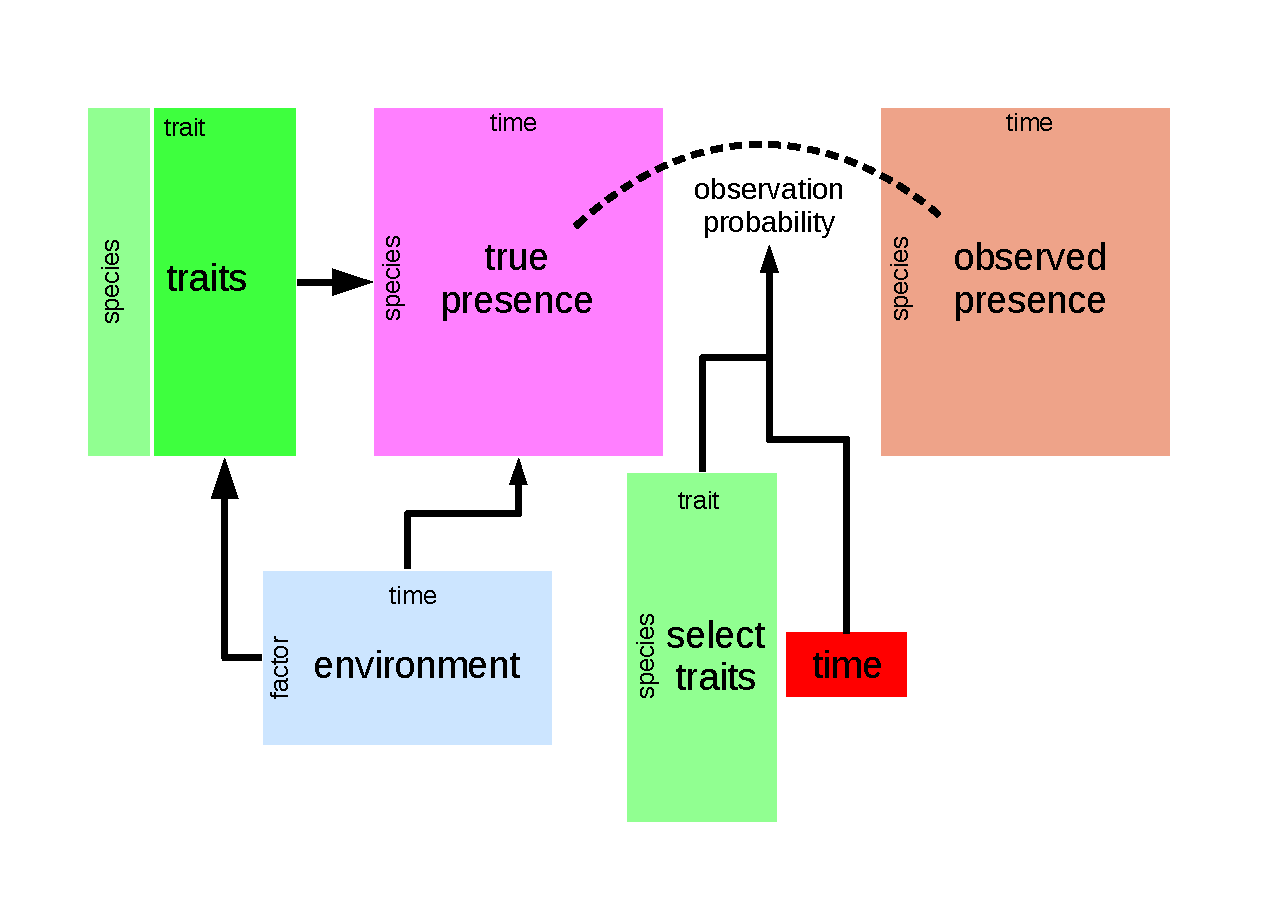
\includegraphics[width=\textwidth,height=0.4\textheight,keepaspectratio=true]{figure/paleo_fourth_corner}
  \caption[Conceptual diagram of the paleontological fourth-courner problem]{Conceptual diagram of the paleontological fourth corner problem. The observed presence matrix (orange) is the empirical presence/absence pattern for all species for all time points; this matrix is an incomplete observation of the ``true'' presence/absence pattern (purple). The estimated true presence matrix is modeled as a function of both environmental factors over time (blue) and multiple species traits (green). Additionally, the affect of environmental factors on species traits are also modeled as traits are expected to mediate the effects of a species environmental context. This diagram is based partially on material presented in \citet{Brown2014c} and \citet{Warton2015a}.}
  \label{fig:concept_fourth_corner}
\end{figure}

% 4th corner as similar but different lens
Fourth-corner modeling is an approach to explaining the patterns of either species abundance or presence/absence as a product of species traits, environmental factors, and the interaction between traits and environment \citep{Brown2014c,Warton2015a,Pollock2012,Jamil2013}; effectively uniting species distribution modeling (SDMs) with trait-based community assembly (CATS, MaxEnt). In modern ecological studies, what is being modeled is species occurrences at localities distributed across a region \citep{Pollock2012,Jamil2013}. In this study, what is being modeled is the pattern of species occurrence over time for most of the Cenozoic in North America (Fig. \ref{fig:concept_fourth_corner}). By incorporating an additional dimension (time) to the fourth-corner framework we can gain better inference of how an instantaneous species pool (i.e. the Modern) is assembled over time. These two approaches, modern and palentologicial, are different views of the same three-dimensional pattern: species at localities over time. The temporal limitations of modern ecological studies and difficulties with uneven spatial occurrences of fossils in paleontological studies means that these approaches are complimentary but reveal different patterns of how species are distributed in time and space.

All observations, paleontological or modern, are made with uncertainty. With presence/absence data this uncertainty comes from now knowing if an absence is a ``true'' absence or just a failure to observe \citep{Royle2008,Royle2005,Foote1999a,Foote2001,Lloyd2011,Wang2016b}. For paleontological data, the incomplete preservation of whatever species were present into fossil form combined with incomplete sampling of what organisms were actually fossilized means that the true times of origination or extinction may not be observed \citep{Foote1999a,Foote2001,Wang2015,Wang2016b}.

Ultimately, the goals of this analysis are to understand when are unique ecotypes enriched or depleted in the North American mammal regional species pool and how changes in ecotypic diversity are related to changes in species' environmental context. In the analyses done here, many covariates which describe both a species' macroecology and its environmental context are considered. In order to analyze this complex and highly structured data set, I developed a hierarchal Bayesian model combing the forth-corner modeling approach with a model of an observation-occurrence or observation-origination-extinction process. The complexity and nuance inherent in questions that are focus of this study, it is possible to consider and test a large number of possible hypotheses. The hierarchical Bayesian modeling approach used here is appropriate for mitigating complications arising from both this complexity and the plethora of testable hypotheses (e.g. multiple comparisons, garden of forking paths) \citep{Gelman2013d,Gelman2012a,Gelman2014}.


\end{document}
